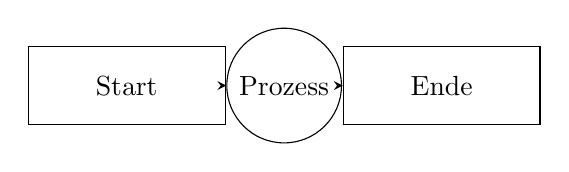
\begin{tikzpicture}[node distance=2cm, >=stealth]

% Knoten (Box, Kreis)
\node[draw, rectangle, minimum width=2.5cm, minimum height=1cm] (A) {Start};
\node[draw, circle, right of=A] (B) {Prozess};
\node[draw, rectangle, right of=B, minimum width=2.5cm, minimum height=1cm] (C) {Ende};

% Verbindungen
\draw[->] (A) -- (B);
\draw[->] (B) -- (C);

\end{tikzpicture}

\begin{tikzpicture}[
    >=stealth,
    block/.style={draw, circle, minimum size=2.6cm},
]

% Radius der äußeren Kreise der ersten Ebene
\def\rA{4}

% Radius der zweiten Ebene um AddOns
\def\rB{3}

% -----------------------------------------
% Erste Ebene (SimLib im Zentrum)
% -----------------------------------------

% SimLib – hellrot
\node[block, fill=red!20] (simlib) at (0,0) {SimLib};

% Komponenten, AddOns, Webexport (wie Diagramm 1)
\node[block, fill=green!20]  (komp)   at (90:\rA)  {Komponenten};
\node[block, fill=cyan!20]   (addons) at (210:\rA) {AddOns};
\node[block, fill=yellow!20] (web)    at (330:\rA) {Webexport};

% Verbindungen Ebenen 1
\draw[->] (simlib) -- (komp);
\draw[->] (simlib) -- (addons);
\draw[->] (simlib) -- (web);

% -----------------------------------------
% Zweite Ebene (um AddOns herum)
% -----------------------------------------

% Drei symmetrische AddOns-Abhängigkeiten (120° Abstand)
\node[block, fill=cyan!20]   (toolw)    at ($(addons)+(90:\rB)$)  {ToolWizard};
\node[block, fill=green!20]  (robotw)   at ($(addons)+(210:\rB)$) {RobotWizard};
\node[block, fill=orange!20] (machinew) at ($(addons)+(330:\rB)$) {MachineWizard};

% Verbindungen AddOns → zweite Ebene
\draw[->] (addons) -- (toolw);
\draw[->] (addons) -- (robotw);
\draw[->] (addons) -- (machinew);

\end{tikzpicture}